% NOTE:
% latexmk -shell-escape -pvc slides.tex # Watches and compiles on each change.
% latexmk -c slides.tex   # Clean the temporal files.

% NOTE: 
% the minted package doesn't play well with the bibliography!


\documentclass[aspectratio=169]{beamer}

\setbeamertemplate{footline}[frame number]
\beamertemplatenavigationsymbolsempty

% NOTE: Only use numeric for references' style!
\usepackage[backend=biber,style=numeric]{biblatex}
\usepackage{booktabs}
\usepackage{caption}
\usepackage{graphicx}
\usepackage{hyperref}
\usepackage{longtable}
\usepackage{siunitx}
\usepackage{subcaption}

\addbibresource{slides.bib}  

\captionsetup[figure]{labelformat=empty}

\hypersetup{
    colorlinks,
    allcolors=.,
    urlcolor=blue,
}


\title{Notes on processing large amounts of Earth Observation data}

\author{Alber S\'{a}nchez \href{mailto:alber.ipia@inpe.br}
{alber.ipia@inpe.br}\newline
Guilherme Mataveli}
\institute{
  
\includegraphics[width=4cm,keepaspectratio]{logos/trees-color-h_2.png}
  
\includegraphics[width=1.8cm,keepaspectratio]
  {logos/logoinpe-azul-menor.png} \\
  Research assistant - TreesLab\\National Institute for Space Research - INPE\\
  Brazil
}
\date{\today}



\begin{document}



\frame{\titlepage}

\begin{frame}[allowframebreaks]
    \frametitle{Overview}
    \tableofcontents
\end{frame}



\section{Introduction}



\begin{frame}
    Introduction.
\end{frame}

% \begin{frame}
%     \frametitle{Two stages: developing and processing}
% \end{frame}



\section{Computing concepts}



\begin{frame}
    Computing concepts.
\end{frame}

\begin{frame}
    \frametitle{Hardware}
    \begin{itemize}
        \item Processor.
        \item Memory.
        \item Disc (Input\/Output, I/O).
        \item Graphic User Interface (GUI).
        \item Console, terminal, shell, tty.
        \item Client, server.
    \end{itemize}
\end{frame}

\begin{frame}
    \frametitle{Software}
\end{frame}

\begin{frame}
    \frametitle{Map - Reduce}
\end{frame}

\begin{frame}
    \frametitle{Resources}
    \begin{columns}
        \begin{column}{0.5\textwidth}
            \begin{itemize}
                \item \href{https://thecrashcourse.com/topic/computerscience/}
                    {Computer Science} by Crash Course.
            \end{itemize}
        \end{column}
        \begin{column}{0.5\textwidth}
            \begin{figure}
                \centering
                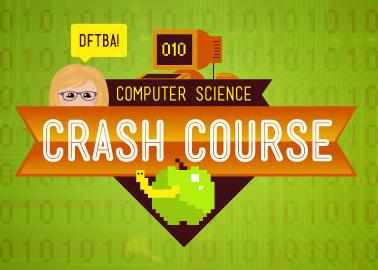
\includegraphics[scale=0.4]
                {img/crash_course_computer_science.jpg}
            \end{figure}
        \end{column}
    \end{columns}
\end{frame}



\section{Linux}



\begin{frame}
    Linux.
\end{frame}

\begin{frame}[allowframebreaks]
    \frametitle{Basic Bash commands}
    \begin{center}
\begin{longtable} { l l }
\hline
Command & Explanation \\
\hline\hline
    \verb|whoami| & What is the current user name (Who am I?).\\
    \verb|pwd|    & Print working directory (Where am I?). \\
    \verb|ls|     & List directory contents. \\
    \verb|cd|     & Change working directory. \\
    \hline
    \verb|man|    & Display manual pages. \\
    \verb|help|   & Display information about commands. \\
    \verb|apropos| & Search the manuals and descriptions. \\
    \hline
    \verb|rm|     & Remove files or directories. \\
    \verb|cp|     & Copy files or directories. \\
    \verb|mv|     & Move (rename) files. \\
    \verb|mkdir|  & Make directories. \\
    \hline
    \verb|less|   & Open a file for reading. \\
    \verb|nano|   & Simple text editor. \\
    \verb|vim|     & Text editor. \\
    \verb|vimtutor| & The Vim tutor. \\
    \hline
    \verb|wget| & Download data from the Internet. \\
    \verb|rsync| & Backup and file copying tool. \\
    \verb|ssh| & Remote login client. \\
    \verb|scp| & Secure file copy. \\
\hline
\end{longtable}
\end{center}

\end{frame}

\begin{frame}
    \frametitle{Resources}
    \begin{columns}
        \begin{column}{0.5\textwidth}
            \begin{itemize}
                \item Webpages: \href{https://linuxjourney.com/}{Linux Journey}.
                \item Books: 
                    \begin{itemize}
                        \item Linux basics for Hackers~\cite{occupytheweb2018}.
                        \item The Linux Command Line~\cite{shotts2019}.
                        \item Unix and Linux System Administration 
                            Handbook~\cite{mackin2017}.
                    \end{itemize}
                \item Courses: 
                    \href{https://training.linuxfoundation.org/training/introduction-to-linux/}
                    {Linux Foundation (LFS101)}.
                \item Videos: 
                    \begin{itemize}
                        \item \href{https://www.learnlinux.tv/linux-commands-for-beginners/}
                            {Linux Commands for Beginners} by Learn Linux TV.
                        \item \href{https://www.learnlinux.tv/linux-essentials/}
                            {Linux Crash Course} by Learn Linux TV.
                        \item \href{https://www.youtube.com/watch?v=px8D72loRVg&list=PLSmXPSsgkZLuJKJhvL1U384aHesbVDekO}
                            {The Linux Command Line Ultimate Tutorial} by 
                            Average Linux User.
                    \end{itemize}
            \end{itemize}
        \end{column}
        \begin{column}{0.5\textwidth}
            \begin{figure}
                \centering
                
\includegraphics[scale=0.6]{logos/tux.png}
            \end{figure}
        \end{column}
    \end{columns}
\end{frame}



\section{Scripting}



\subsection{Bash}



\begin{frame}
    Bash scripting.
\end{frame}

\begin{frame}
    \frametitle{Resources}
    \begin{columns}
        \begin{column}{0.5\textwidth}
            \begin{itemize}
                \item Books: The Linux Command Line~\cite{shotts2019}.
                \item Tutorials: \href{https://swcarpentry.github.io/shell-novice/}
                    {The Unix Shell} by Software Carpentry.
                \item Videos: 
                    \href{https://www.youtube.com/watch?v=2733cRPudvI&list=PLT98CRl2KxKGj-VKtApD8-zCqSaN2mD4w}
                    {Bash Scripting on Linux} by Learn Linux TV.
            \end{itemize}
        \end{column}
        \begin{column}{0.5\textwidth}
            \begin{figure}
                \centering
                
\includegraphics[scale=0.05]{logos/bash.png}
            \end{figure}
        \end{column}
    \end{columns}

\end{frame}


\subsection{How to process data without a GUI}


\begin{frame}
    How to process data without a GUI.
\end{frame}

\begin{frame}
    \frametitle{Data Science at the Command Line\cite{janssens2021}}
    \begin{columns}
        \begin{column}{0.5\textwidth}
            \begin{itemize}
                \item Get data from websites, APIs, databases, and
                    spreadsheets; scrub text, CSV, HTML, XML, JSON.
                \item Explore data, compute statistics, create
                    visualizations.
                %\item Manage your data science workflow.
                \item Create your own tools, re-use code.
                \item Parallelize and distribute data pipelines.
                \item Model data with dimensionality reduction, regression, and
                    classification algorithms.
                \item Command line from Python, Jupyter, R, RStudio, Apache
                    Spark.
                \item Read online~\href{https://jeroenjanssens.com/dsatcl}
                    {here}.
            \end{itemize}
        \end{column}
        \begin{column}{0.5\textwidth}
            \begin{figure}
                \centering
                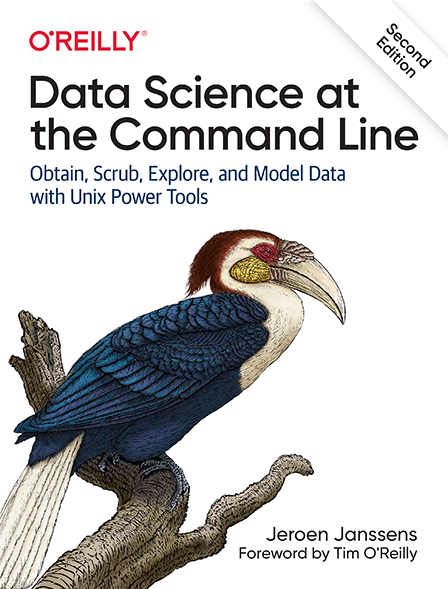
\includegraphics[scale=0.3]
                {img/data_science_at_the_command_line.png}
            \end{figure}
        \end{column}
    \end{columns}
\end{frame}

\begin{frame}
    \frametitle{GRASS GIS}
    \begin{columns}
        \begin{column}{0.5\textwidth}
            \begin{itemize}
                \item Geographic Resources Analysis Support System.
                \item Vector and raster geospatial data management, 
                    geoprocessing, spatial modelling, and visualization.
                \item Free, Libre, and Open Source Software.
                \item Docker container.
                \item Open Source GIS: A GRASS GIS Approach~\cite{neteler2008}.
            \end{itemize}
        \end{column}
        \begin{column}{0.5\textwidth}
            \begin{figure}
                \centering
                
\includegraphics[scale=0.5]{logos/grassgis.png}
            \end{figure}
        \end{column}
    \end{columns}
\end{frame}

\begin{frame}
    \frametitle{Orfeo ToolBox (OTB)}
    \begin{columns}
        \begin{column}{0.5\textwidth}
            \begin{itemize}
                \item OTB is a set of state-of-the-art remote sensing tools.
                \item It is FOSS (Free Open Source Software).
                \item Wide variety of applications available: from 
                    ortho-rectification or pansharpening, all the way to 
                    classification, SAR processing, and much more!
                \item \url{www.orfeo-toolbox.org}
            \end{itemize}
        \end{column}
        \begin{column}{0.5\textwidth}
            \begin{figure}
                \centering
                
\includegraphics[scale=0.8]{logos/orfeo-toolbox.png}
            \end{figure}
        \end{column}
    \end{columns}
\end{frame}

\begin{frame}
    \frametitle{GDAL programs/utilities}
    \begin{columns}
        \begin{column}{0.5\textwidth}
            \begin{itemize}
                \item GDAL is a translator FOSS library for raster and vector 
                    geospatial data.
                \item It presents a single raster abstract data model and
                    single vector abstract data model to the calling
                    application for all supported formats.
                \item It also comes with a variety of useful command line
                    utilities for data translation and processing.
                \item Docker container.
                \item \footnotesize{\url{https://gdal.org/programs/index.html}}
                \item \href{https://spatialthoughts.com/courses/mastering-gdal-tools/}{Mastering GDAL tools}.
            \end{itemize}
        \end{column}
        \begin{column}{0.5\textwidth}
            \begin{figure}
                \centering
                
\includegraphics[scale=0.2]{logos/gdalicon.png}
            \end{figure}
        \end{column}
    \end{columns}
\end{frame}


\subsection{R}


\begin{frame}
    R language and environment for statistical computing.
\end{frame}

\begin{frame}
    \frametitle{Make script take parameters}
\end{frame}

\begin{frame}
    \frametitle{Iteration}
    Recomended reading:
    \begin{itemize}
        \item Iteration, chapter 26~\cite{wickham2023a}.
        \item Functionals, chapter 9~\cite{wickham2019}.
    \end{itemize}
\end{frame}

\begin{frame}
    \frametitle{Parallelize code}
\end{frame}

\begin{frame}
    \frametitle{Resources}
    \begin{itemize}
        \item Tutorials: \href{https://www.w3schools.com/r/default.asp}
            {R Tutorial} by w3schools.
        \item Books: 
            \begin{itemize}
                \item An introduction to R~\cite{venables2024},
                \item Advanced R~\cite{wickham2015a}.
            \end{itemize}
    \end{itemize}
\end{frame}



% \subsection{Python}



\section{Virtualization and containerization}



\begin{frame}
    Virtualization and containerization.
\end{frame}

\begin{frame}
    \frametitle{Virtualization}
    \begin{columns}
        \begin{column}{0.5\textwidth}
            \begin{itemize}
                \item A host is a piece of hardware.
                \item A virtual machine takes pieces of host's CPU, memory, and
                    disc and simulates new hardware.
                \item A software called Hypervisor takes care of virtual
                    machines in a host.
                \item VirtualBox and VMware are popular virtualization 
                    software.
            \end{itemize}
        \end{column}
        \begin{column}{0.5\textwidth}
            \begin{figure}
                \centering
                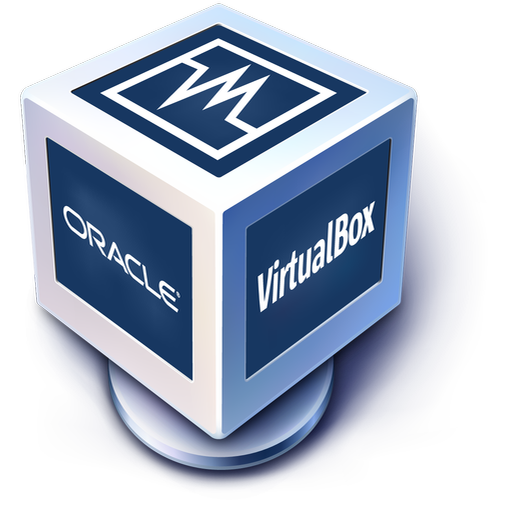
\includegraphics[scale=0.2]{logos/virtualbox.png}
                
\includegraphics[scale=0.2]{logos/vmware.jpg}
            \end{figure}
        \end{column}
    \end{columns}
\end{frame}

\begin{frame}
    \frametitle{Containerization}
    \begin{columns}
        \begin{column}{0.5\textwidth}
            \begin{itemize}
                \item A host is a piece of hardware.
                \item A virtual machine takes pieces of host's CPU, memory, and
                    disc and simulates new hardware but it's able to share them
                    with other host's processes.
                \item Reproducible, lightweight environments for processes to
                    run.
                \item You're probably using them without knowing it.
                \item Docker and Podman are software for containerization.
            \end{itemize}
        \end{column}
        \begin{column}{0.5\textwidth}
            \begin{figure}
                \centering
                
\includegraphics[scale=0.25]{logos/docker-logo.jpg}
                
\includegraphics[scale=0.3]{logos/podman-logo.png}
            \end{figure}
        \end{column}
    \end{columns}
\end{frame}

\begin{frame}
    \frametitle{Docker}
    \begin{columns}
        \begin{column}{0.5\textwidth}
            \begin{itemize}
                \item An image is a template for creating containers.
                \item Images are immutable. Once created, they can't be
                    changed.
                \item A container is an instance of an image.
                \item Docker has a repository of images called 
                    \href{https://hub.docker.com/}{dockerhub}.
            \end{itemize}
        \end{column}
        \begin{column}{0.5\textwidth}
            \begin{figure}
                \centering
                
\includegraphics[scale=0.5]{logos/docker-logo.jpg}
            \end{figure}
        \end{column}
    \end{columns}
\end{frame}

\begin{frame}
    \frametitle{Rocker project}
    \begin{columns}
        \begin{column}{0.5\textwidth}
            \begin{itemize}
                \item Docker containers for the R 
                    Environment.
                \item Docker images of r-base, rstudio, shiny, CUDA,
                    geospatial.
                \item Portable, sandboxed, transparent, community optimized,
                    versioned, extensible~\cite{boettiger2017}.
                \item Applications include 
                    %development-debugging-testing,
                    data processing,
                    %deployment and continous delivery, create and
                    share computing environments (HPC), teaching, packaging
                    research reproducibility ~\cite{nust2020}.
                \item Rocker project web page \url{https://rocker-project.org}.
            \end{itemize}
        \end{column}
        \begin{column}{0.5\textwidth}
            \begin{figure}
                \centering
                
\includegraphics[scale=0.25]{logos/rocker.png}
            \end{figure}
        \end{column}
    \end{columns}
\end{frame}

\begin{frame}
    \frametitle{Reproducible development environments}
    \begin{itemize}
        \item How do I get the same environment during developing and 
            processing?
    \end{itemize}
\end{frame}



\section{Platforms}



\subsection{sepal.io}

\begin{frame}
    System for Earth Observation Data Access, Processing and Analysis for Land
    Monitoring - SEPAL.
\end{frame}

\begin{frame}
    \frametitle{SEPAL}
    \begin{columns}
        \begin{column}{0.5\textwidth}
            \begin{itemize}
                \item Cloud computing-based platform for autonomous land 
                    monitoring using remote sensing data.
                \item This platform allows users to access powerful 
                    cloud-computing resources to query, access and process 
                    satelllite data quickly and efficiently for conducting 
                    advanced analysis.
                \item It is part of OpenForis.
            \end{itemize}
        \end{column}
        \begin{column}{0.5\textwidth}
            \begin{figure}
                \centering
                
\includegraphics[scale=0.4]{logos/sepal.png}
                
\includegraphics[scale=0.8]{logos/openforis.png}
            \end{figure}
        \end{column}
    \end{columns}
\end{frame}

\begin{frame}
    \frametitle{Setup}
    Create accounts at:
    \begin{itemize}
        \item SEPAL.
        \item Google Earth Engine.
        \item Collect Earth Engine.
        \item NICFI-PlanetLab data.
    \end{itemize}
\end{frame}

\begin{frame}
    \frametitle{Get data}
    \begin{itemize}
        \item Connect SEPAL to Google Earth Engine.
        \item Connect SEPAL to NICFI-PlanetLab (Norway's International Climate 
            and Forest Initiative).
    \end{itemize}
\end{frame}

\begin{frame}
    \frametitle{Recipes}
    \begin{itemize}
        \item Quickly and efficiently query and process satellite data.
        \item A recipe is a record of steps and parameters used to make a 
            data set (e.g. classification).
        \item Access GEE imagery catalog and run planetary-scale analysis 
            without a line of code.
        \item Recipes include creating mosaics (optical, radar, planet), 
            supervised classifications (of images or time series).
    \end{itemize}
\end{frame}

\begin{frame}
    \frametitle{Modules}
    \begin{itemize}
        \item GIS tools that complement SEPAL's recipes.
        \item Based on advanced GIS libraries.
    \end{itemize}
\end{frame}

\begin{frame}
    \frametitle{Workflows}
    \begin{itemize}
        \item Combinations of Recipes, modules, and tools to perform complex
            data analysis.
    \end{itemize}
\end{frame}

\begin{frame}
    \frametitle{CLI utilities}
    \begin{itemize}
        \item Command Line Interface utilities.
        \item GDAL, Google Drive, GEE, GuidosToolbox Workbench, Open Foris 
            Geospatial Toolbox, Orfeo Toolbox, Python, R code.
        \item IDEs.
    \end{itemize}
\end{frame}

\begin{frame}
    \frametitle{IDEs}
    \begin{itemize}
        \item Integrated Development Environments.
        \item JupyterLab.
        \item Jupyter Notebook.
        \item RStudio.
    \end{itemize}
\end{frame}

\begin{frame}
    \frametitle{Start a machine}
\end{frame}

\begin{frame}
    \frametitle{Get data}
\end{frame}

\begin{frame}
   \frametitle{Start an R-spatial container} 
\end{frame}

\begin{frame}
   \frametitle{Get root password} 
\end{frame}


\subsection{Google Earth Engine}

\begin{frame}
    Google Earth Engine.
\end{frame}


\subsection{INPE}

\begin{frame}
    National Institute for Space Research in Brazil - INPE.\\
    \url{https://data.inpe.br}
\end{frame}

\begin{frame}
    \frametitle{Base de Informações Georeferenciadas - BIG}
    \begin{itemize}
        \item Hospedar programas e projetos que producem dados.
        \item Os dados do INPE: \url{https://data.inpe.br/stac/browser}
        \item O servidor de mapas BDC : \url{https://data.inpe.br/big/geoserver}
        \item Contato: \href{mailto:[data.support@inpe.br]}{data.support@inpe.br}
    \end{itemize}
\end{frame}

\begin{frame}
    \frametitle{Base de Informações Georeferenciadas - BIG}
    \begin{itemize}
        \item Ambiente operacional (24/7).
        \item Infraestrutura para atender projetos institucionais.
        \item Instancias de processamento sob demanda:
            \begin{itemize}
                \item (2vCPUs + 8GB RAM) - (256vCPUs + 1TB RAM)
                \item GPUs A100 e H100 (em preparação)
            \end{itemize}
        \item Contato: \href{mailto:[data.support@inpe.br]}{data.support@inpe.br}
    \end{itemize}
\end{frame}

\begin{frame}
    \frametitle{Brazil Data Cubes - BDC}
    \begin{itemize}
        \item Os dados do BDC: \url{https://data.inpe.br/bdc/explorer}
        \item O servidor de mapas BDC : \url{https://data.inpe.br/bdc/geoserver}
        \item O BDC Lab: \url{https://data.inpe.br/bdc/lab}
        \item Contato: \href{mailto:[data.support@inpe.br]}{data.support@inpe.br}
    \end{itemize}
\end{frame}

\begin{frame}
        \frametitle{Infraestrutura digital BIG BDC na COIDS}
        \begin{itemize}
            \item \url{https://data.inpe.br/iam}
            \item \url{https://data.inpe.br/big/geonetwork}
            \item \url{https://data.inpe.br/big/geoserver}
            \item \url{https://data.inpe.br/big/nextcloud}
            \item \url{https://data.inpe.br/stac/browser}
            \item \url{https://data.inpe.br/bdc/stac}
            \item \url{https://data.inpe.br/bdc/wtss}
            \item \url{https://data.inpe.br/bdc/wlts}
            \item \url{https://data.inpe.br/bdc/geoserver}
            \item \url{https://data.inpe.br/bdc/explorer}
            \item \url{https://data.inpe.br/bdc/terracollect}
            \item \url{https://data.inpe.br/bdc/lab}
            \item \url{https://data.inpe.br/queimadas/bdq}
            \item \url{https://data.inpe.br/queimadas/geoserver}
            \item \url{https://data.inpe.br/queimadas/situacao_atual}
        \end{itemize}
\end{frame}

\begin{frame}
    \frametitle{Infraestrutura compartilhada de pesquisa na DIOTG (experimental)}
    \begin{itemize}
        \item Jupyter
        \item Python
        \item Rstudio
        \item \textit{R}
        \item QGIS
        \item Nextcloud
        \item PostGRESQL
        \item Virtual machines
        \item Metview
    \end{itemize}
\end{frame}

\begin{frame}
    \frametitle{BDC-Lab DIOTG}
    \begin{itemize}
        \item Atividades de capacitação.
            \begin{itemize}
                \item Oficina BIG/Queimadas.
                \item BIG TechTalks.
                \item PG-CAP CAP-419 CAP-395
                \item PG-SER SER-347 SER-350
            \end{itemize}
        \item Pesquisas.
        \item Recursos disponiveis.
    \end{itemize}
\end{frame}


\section{Test case: sepal.io}



\begin{frame}
    Test case: sepal.io
\end{frame}

\begin{frame}
    \frametitle{Script for...}
    \begin{itemize}
        \item Suppose we have an R script for computing...
    \end{itemize}
\end{frame}



%%%%%%%%%%%%%%%%%%%%%%%%%%%%%%%%%%%%%%%%%%%%%%%%%%%%%%%%%%%%%%%%%%%%%%%%%%%%%%

\begin{frame}
    \frametitle{Take home message}
\end{frame}

\begin{frame}[allowframebreaks]
	\frametitle{References}
	\printbibliography
\end{frame}

\end{document}

